% ReCoMER - CVPR 2026 format
% Rebuilt from the Word draft; equations typeset natively, citations via BibTeX.

\documentclass[10pt,twocolumn,letterpaper]{article}

\usepackage[review]{cvpr}      % REVIEW version (with line numbers)
% \usepackage{cvpr}             % CAMERA-READY version
% \usepackage[pagenumbers]{cvpr} % arXiv version

%% This file contains a number of tweaks that are typically applied to the main document.
%% They are not enabled by default, but can be enabled by uncommenting the relevant lines.


%%
%% Official support for 2-column teaser figure
%%
\usepackage{cuted} %< for strip environment

%%
%% For auto-referencing of figures (see fig/teaser.tex and \label{} therein) 
%%
\usepackage{currfile} %< for \currfilebase macro

%%
%% caption and (global) spacing overrides
%%
\usepackage{caption} %< for "\captionof" commands (teaser)
% \setlength{\abovecaptionskip}{.5em} % space above caption
% \setlength{\belowcaptionskip}{1em} % space below caption

%%
%% Inline annotations; for predefined colors, refer to "dvipsnames" in the xcolor package:
%% https://tinyurl.com/overleaf-colors
%%
\newcommand{\red}[1]{{\color{red}#1}}
\newcommand{\todo}[1]{{\color{red}#1}}
\newcommand{\TODO}[1]{\textbf{\color{red}[TODO: #1]}}
%%
%% Disable for camera ready / submission by uncommenting these lines:
%%
% \renewcommand{\TODO}[1]{}
% \renewcommand{\todo}[1]{#1}

%%
%% Work harder in optimizing text layout. Typically shrinks text by 1/6 of page, enable
%% it at the very end of the writing process, when you are just above the page limit.
%%
% \usepackage{microtype}

%%
%% Fine-tune paragraph spacing.
%%
% \renewcommand{\paragraph}[1]{\vspace{.5em}\noindent\textbf{#1.}}

%%
%% Globally adjusts space between figure and caption.
%%
% \setlength{\abovecaptionskip}{.5em}

%%
%% Allows "the use of \paper to refer to the project name"
%% with automatic management of space at the end of the word.
%%
% \usepackage{xspace}
% \newcommand{\paper}{ProjectName\xspace}

%%
%% Commonly used math definitions.
%%
% \DeclareMathOperator*{\argmin}{arg\,min}
% \DeclareMathOperator*{\argmax}{arg\,max}

%%
%% Tighten underline.
%%
% \usepackage{soul}
% \setuldepth{foobar}

%%
%% Reconfigure paragraph (tweaks spacing)
%%


% Times text font under Tectonic/XeTeX (times.sty falls back to Latin Modern otherwise)
\usepackage{fontspec}
\setmainfont{texgyretermes-regular.otf}[
  BoldFont = texgyretermes-bold.otf,
  ItalicFont = texgyretermes-italic.otf,
  BoldItalicFont = texgyretermes-bolditalic.otf]
\usepackage{microtype}

\definecolor{cvprblue}{rgb}{0.21,0.49,0.74}
\usepackage[pagebackref,breaklinks,colorlinks,allcolors=cvprblue]{hyperref}

\def\paperID{*****} % TODO: enter the Paper ID when assigned
\def\confName{CVPR}
\def\confYear{2026}

\title{ReCoMER: Reliability and Context Modeling for Multimodal\\Conversational Emotion Recognition}

\author{Anonymous CVPR submission\\
Paper ID \paperID}

\usepackage{amsmath,amssymb}
\usepackage{booktabs}
\usepackage{multirow}
\DeclareMathOperator*{\argmaxop}{arg\,max}
\newcommand{\M}{\mathcal{M}}
\newcommand{\Hist}{\mathcal{H}}
\newcommand{\Kset}{\mathcal{K}}
\newcommand{\sg}{\mathrm{sg}}
\newcommand{\ind}{\mathbb{I}}
\newcommand{\softmax}{\mathrm{softmax}}
\newcommand{\mean}{\mathrm{mean}}
\newcommand{\sd}{\mathrm{sd}}
\newcommand{\clip}{\mathrm{clip}}

\begin{document}
\maketitle

%%%%%%%%% ABSTRACT
\begin{abstract}
Multimodal conversational emotion recognition requires a model to decide not only how to combine text, audio and vision, but also whether historical context and an external prediction should be trusted for the current utterance.
We present ReCoMER, a reliability- and context-aware framework that combines the MHnoU predictor with the independent cRBEF expert.
MHnoU integrates feedback-conditioned context reassessment, Shapley-anchored bounded evidence routing, and null-candidate history abstention; cRBEF constructs prior-relative audio-visual evidence and regulates it with a reliability gate.
A bounded class-wise fusion module then combines the two complete predictions while preserving an exact equal-weight fallback.
On the frozen formal M3ED test, ReCoMER reaches 58.00\% WF1, improving over matched equal-weight fusion by 0.607 percentage points.
Module-isolation experiments show conditional gains on MOSEI, MELD and IEMOCAP, while also exposing negative or neutral regimes.
The framework separates prediction, history admission, contribution estimation and expert fusion, making both its improvements and its failure boundaries auditable.
\end{abstract}

%%%%%%%%% 1. INTRODUCTION
\section{Introduction}
\label{sec:intro}

Multimodal emotion recognition (MER) in conversations aims to identify the emotion of each utterance by integrating textual, acoustic and visual cues with conversational context~\cite{majumder2019dialoguernn,poria2019meld,zhao2022m3ed}.
Spoken words carry semantic content, while prosody and facial expressions describe how that content is expressed, and previous utterances help disambiguate emotional changes across a dialogue~\cite{busso2008iemocap,zadeh2018cmumosei}.
Effective recognition therefore requires more than combining available features: a model must determine \emph{which} modalities provide useful evidence and \emph{whether} historical information supports the current judgment.
These capabilities matter for empathetic dialogue systems, intelligent tutoring, and human--robot interaction.

\begin{figure}[t]
  \centering
  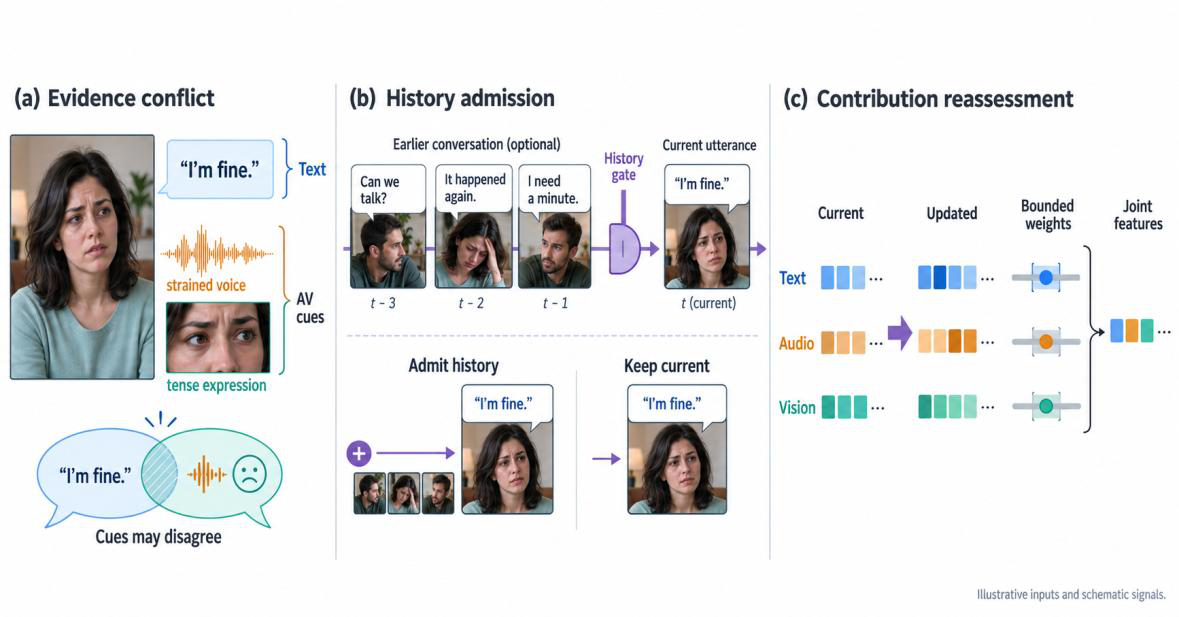
\includegraphics[width=\linewidth]{figures/fig1_motivation.png}
  \caption{\textbf{Motivation for selective context and modality evidence control.}
  (a)~Similar text can receive opposite emotion labels once acoustic and visual evidence is considered, so modality evidence must be weighed per utterance.
  (b)~History can either resolve ambiguity or reinforce an outdated emotional state, so history admission must be selective.
  (c)~Confidence is not contribution: a confident modality may add nothing beyond the other modalities.}
  \label{fig:motivation}
\end{figure}

However, modality contributions and the usefulness of history vary across utterances (Fig.~\ref{fig:motivation}).
A modality may carry clear emotional evidence in one instance but be weak, redundant, or conflicting in another, and predictive confidence alone does not capture this variation~\cite{gao2024eau}.
Historical context introduces a second difficulty: earlier utterances may resolve ambiguity, but they may also reinforce an outdated emotional state~\cite{li2026hiroc}.
Moreover, historical feedback changes the current modality representations and can consequently alter their relative contributions.
These challenges call for coordinated mechanisms that reassess representations after feedback, estimate modality contributions beyond confidence, and explicitly control the admission of historical information.

Existing approaches do not coordinate these decisions.
First, methods that determine modality weights before historical feedback~\cite{li2023dferc} may fail to reassess contributions once context changes the current representations.
Second, confidence-based routing~\cite{fang2025emoe} can favour confident but redundant modalities, because confidence does not measure marginal predictive contribution.
Third, relevance-based history attention~\cite{ghosal2019dialoguegcn,ghosal2020cosmic} selects related utterances but, without an explicit abstention mechanism, may still inject unhelpful or outdated emotional information.
Consequently, modality dominance and harmful historical updates can persist even when fusion is adaptive.

To address these challenges, we equip the MHnoU predictor with three coordinated mechanisms.
Feedback-Conditioned Context Reassessment (FCCR) retrieves historical information, incorporates admitted feedback, and reassesses modality contributions from the \emph{updated} representations.
Shapley-Anchored Bounded Evidence Routing (SABER) trains a contribution predictor with sample-level Shapley targets~\cite{shapley1953value} and maps the predicted scores to bounded deviations from uniform weights, constraining reliance on any single modality.
Null-Candidate History Abstention (NCHA) lets a learned null candidate compete with real historical slots during attention, so the model can reject the entire historical update.
A second, complementary perspective is provided by cRBEF: an independently trained audio-visual expert supplies prior-relative nonverbal evidence, and a reliability gate decides when and how strongly this evidence may adjust the text--audio--visual prediction.
ReCoMER combines the two complete predictions through bounded class-wise correction, starting from their average and preserving an exact equal-weight fallback (Fig.~\ref{fig:framework}).

Our contributions are:
\begin{itemize}
  \item We propose ReCoMER, a framework that combines selective contextual reasoning and complementary evidence assessment through two parallel models and bounded prediction fusion.
  \item We develop MHnoU, integrating FCCR, SABER and NCHA to reassess modality contributions after historical feedback, constrain contribution-guided modality weights, and selectively accept historical updates.
  \item We incorporate cRBEF, which couples text--audio--visual and joint audio--visual predictors through prior-relative evidence and reliability gating, improving the use of informative nonverbal cues while limiting unreliable corrections.
\end{itemize}

%%%%%%%%% 2. RELATED WORK
\section{Related Work}
\label{sec:related}

\paragraph{Multimodal emotion recognition in conversations.}
Recurrent approaches exemplified by DialogueRNN~\cite{majumder2019dialoguernn} track conversational and speaker states; graph-based approaches make utterance and modality relations explicit (MMGCN~\cite{hu2021mmgcn}, M$^3$Net~\cite{chen2023m3net}), DialogueGCN~\cite{ghosal2019dialoguegcn} models speaker dependencies, and COSMIC~\cite{ghosal2020cosmic} injects commonsense knowledge.
Context selection further determines which information enters these representations: ECERC~\cite{zhang2025ecerc} gates evidence--cause interactions, HiRoC~\cite{li2026hiroc} filters historical interactions before aggregation, and DialogueCRN~\cite{hu2021dialoguecrn} performs iterative contextual reasoning; TelME~\cite{yun2024telme} strengthens non-verbal representations by cross-modal distillation.
These methods improve contextual representations but leave history admission implicit; MHnoU instead learns an explicit empty-history candidate that can abstain per sample.

\paragraph{Modality imbalance and contribution estimation.}
Optimization-based methods regulate how modalities are trained: gradient modulation~\cite{peng2022gradientmodulation} rescales modality-specific updates, PMR~\cite{fan2023pmr} rebalances slower-learning modalities with prototypes, and PaSE~\cite{he2026pase} combines prototype alignment with Shapley-based modulation.
Adaptive fusion learns sample-dependent modality weights, differing in supervision target: DF-ERC~\cite{li2023dferc} uses unimodal true-class probabilities, EMOE~\cite{fang2025emoe} derives targets from unimodal errors, and DREAM~\cite{bi2025dream} distills Shapley-based estimates into fusion weights.
MHnoU estimates contributions \emph{after} history feedback and converts them into bounded weight adjustments.

\paragraph{Reliability-aware fusion.}
At the representation level, EAU~\cite{gao2024eau} weights features by estimated unimodal aleatoric uncertainty.
At the prediction level, FINCH~\cite{ovanger2026finch} combines acoustic predictions with spatiotemporal priors in log-probability space, and HiRoC~\cite{li2026hiroc} gates nonverbal residual logits by textual--nonverbal disagreement.
cRBEF belongs to this prediction-level line, but its correction is derived from a separately trained nonverbal posterior expressed relative to an explicit class prior, rather than from learned residual logits inside the conversational model.

%%%%%%%%% 3. METHOD
\section{Method}
\label{sec:method}

\begin{figure*}[t]
  \centering
  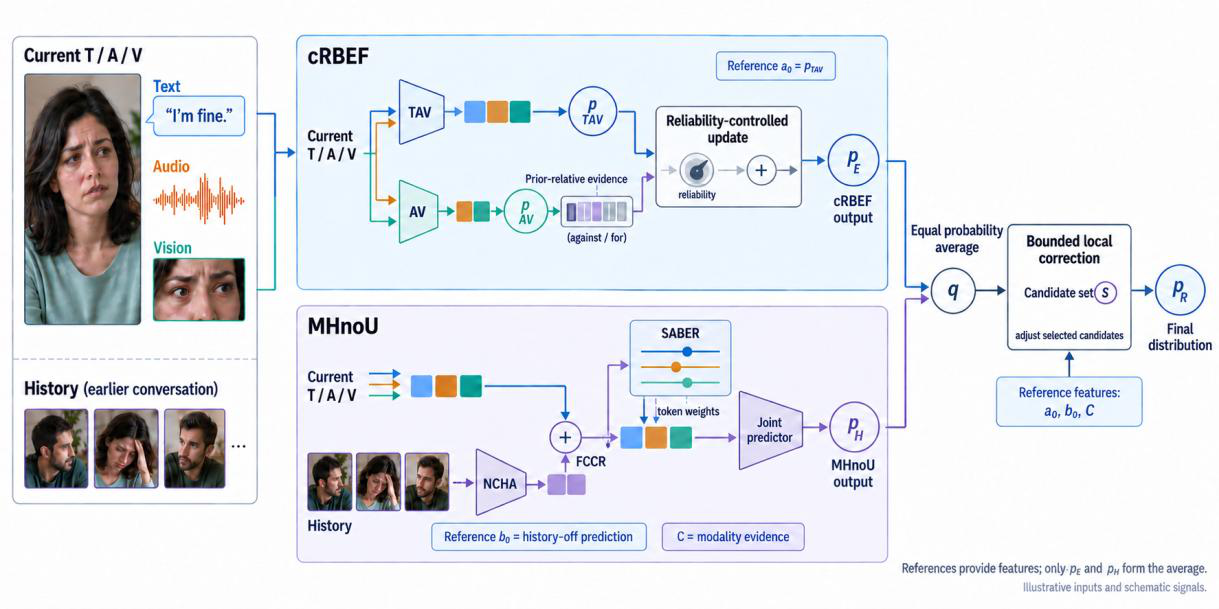
\includegraphics[width=\textwidth]{figures/fig2_framework.png}
  \caption{\textbf{ReCoMER framework overview.}
  Modality-specific encoders (shared between current and historical inputs) produce the current tokens $z_t^m$ and history tokens $h_j^m$ for text, audio and vision.
  In MHnoU (upper path), FCCR lets each current token query its valid historical slots and applies the admitted feedback as a gated residual; NCHA adds a learned null candidate to this attention so the whole historical update can be rejected; SABER predicts Shapley-supervised contribution scores and maps them to bounded routing weights; the routed tokens feed the joint predictor, yielding $p^H$.
  In cRBEF (lower path), a text--audio--visual (TAV) predictor and a text-free audio--visual (AV) predictor produce two distributions; a six-statistic reliability gate scales the prior-relative AV evidence before it corrects the TAV prediction, yielding $p^E$.
  The bounded class-wise fusion module then interpolates between the equal-weight baseline $q$ and a candidate-restricted correction informed by two reference distributions, producing $p^R$ with an exact fallback to equal weighting.}
  \label{fig:framework}
\end{figure*}

\subsection{Task formulation and framework overview}
\label{sec:formulation}

Given an utterance at turn $t$, we predict its emotion label $y$ from current textual, acoustic and visual features and a bounded history window.
The modality set is $\M=\{T,A,V\}$ and $K$ denotes the number of emotion classes.
A current mask $M_t$ and history-slot masks identify available inputs.
MHnoU applies modality-specific encoders, each shared between current and historical features:
\begin{equation}
  z_t^m = E_m(x_t^m), \qquad h_j^m = E_m(x_j^m), \qquad m \in \M=\{T,A,V\}.
  \label{eq:encoders}
\end{equation}
ReCoMER contains two parallel prediction models and an outer fusion module (Fig.~\ref{fig:framework}).
MHnoU coordinates FCCR, SABER and NCHA: its forward path first assesses history admission, incorporates admitted feedback, and routes the updated modality representations.
Independently, cRBEF combines a text--audio--visual predictor with a joint audio--visual predictor.
Bounded class-wise correction then combines the two complete predictions, which are aligned by utterance identifiers and class order.

\subsection{Feedback-Conditioned Context Reassessment}
\label{sec:fccr}

\begin{figure}[t]
  \centering
  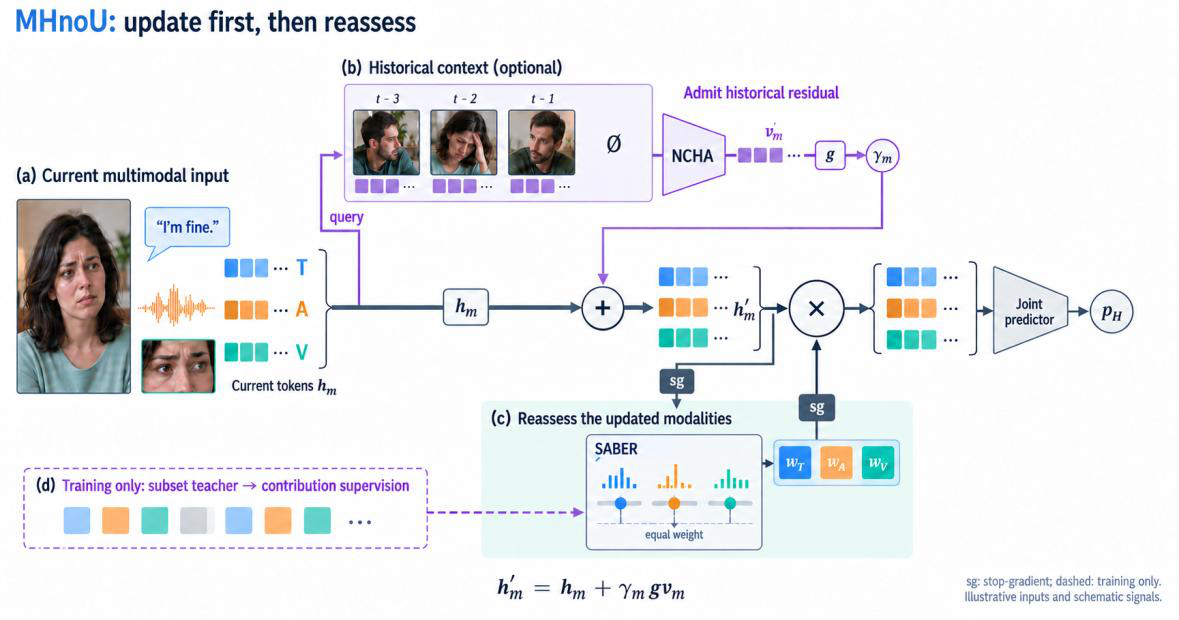
\includegraphics[width=0.94\linewidth]{figures/fig3_mhnou.png}
  \caption{\textbf{MHnoU: history feedback, contribution routing and history admission.}
  Left: the failure mode of a standard history-attention block, which assigns mass to every valid-looking slot.
  Middle: FCCR retrieves historical evidence, applies it as a gated residual, and reassesses the updated modality tokens.
  Right: the admitted feedback feeds SABER's bounded routing and the joint prediction, so contribution estimation always reflects the post-feedback representations.}
  \label{fig:mhnou}
\end{figure}

A standard history-attention block (Fig.~\ref{fig:mhnou}) assigns mass to every valid-looking slot even when a previous utterance is irrelevant or partially observed.
FCCR makes history a conditional correction rather than an unconditional input.
The current utterance and up to three preceding slots are encoded by the same modality-specific encoder, so historical and current vectors share one 192-dimensional space per modality.
For each modality $m$, the current embedding queries only the valid historical slots through scaled dot-product attention~\cite{vaswani2017attention}; the history mask and the per-modality availability mask are multiplied before attention, so a padded slot or a missing modality cannot contribute a value vector.
The feedback-conditioned update is
\begin{equation}
  s_{tj}^m = \frac{\langle W_q^m z_t^m,\, h_j^m\rangle}{\sqrt{d}}, \qquad
  \bar{h}_t^m = \sum_{j\in\Hist_t} \alpha_{tj}^m h_j^m,
  \label{eq:fccr}
\end{equation}
\begin{equation}
  \tilde{z}_t^m = z_t^m + g_t \gamma_m \bar{h}_t^m,
  \label{eq:residual}
\end{equation}
where the first term of the update is the current modality state, the second is the masked history summary, and the per-modality scalar $\gamma_m$, initialized to zero, controls the residual strength.
The null candidate used by NCHA (Sec.~\ref{sec:ncha}) contributes an attention score but no value vector.

After the history decision, each updated modality representation is passed to an auxiliary solo head, giving modality-wise evidence that the router inspects \emph{after} feedback has changed the representation---a closed loop of select, update, reassess:
\begin{equation}
  p^H = \softmax\!\big(F_{\mathrm{joint}}\big(\{\sg(w_m)\,\tilde{z}_t^m\}_{m\in\M},\, M_t\big)\big),
  \label{eq:joint}
\end{equation}
where $\sg$ denotes stop-gradient.
The joint predictor is a two-layer six-head Transformer encoder (feed-forward width 576) with masked attention and masked mean pooling; the modality mask is carried into both, so unavailable tokens neither dilute the representation nor receive an artificial uniform contribution.

\subsection{Shapley-Anchored Bounded Evidence Routing}
\label{sec:saber}

\begin{figure}[t]
  \centering
  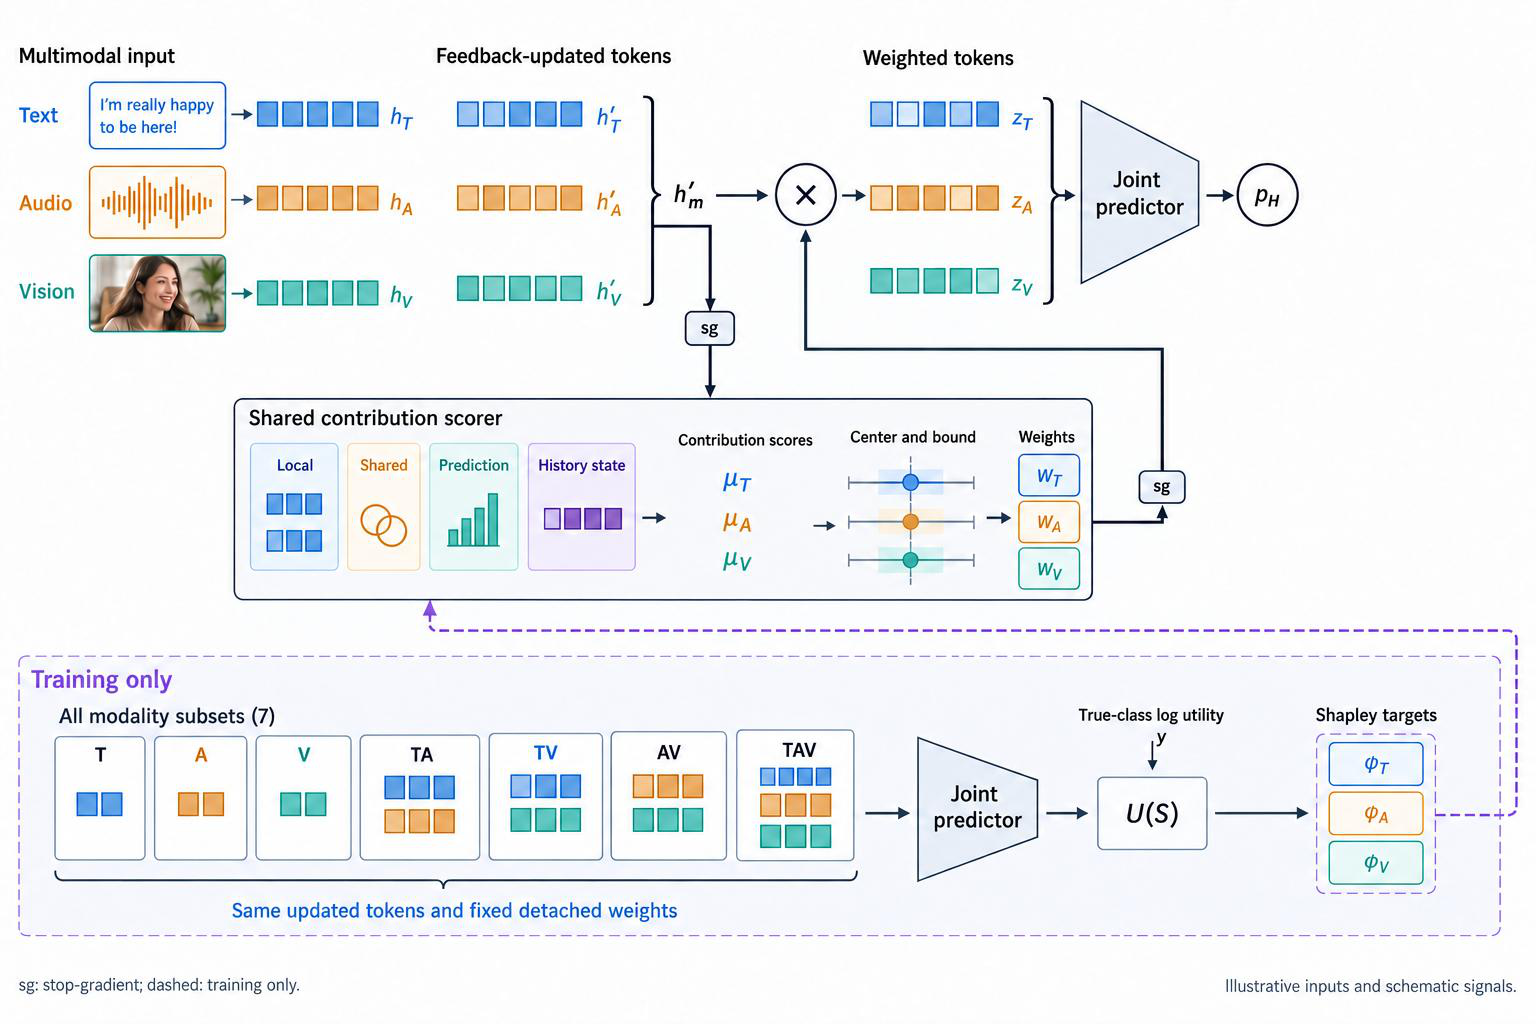
\includegraphics[width=0.94\linewidth]{figures/fig4_saber.png}
  \caption{\textbf{SABER contribution supervision and bounded routing.}
  Left: uniform averaging or a free gate cannot explain per-utterance modality usefulness.
  Middle: the teacher evaluates all nonempty modality subsets to obtain exact Shapley targets, which supervise the contribution scorer $\mu$ after standardization.
  Right: the predicted scores are centered and mapped through the bounded mapping of Eq.~\eqref{eq:bounded}, keeping deployment weights inside a narrow interval around uniform.}
  \label{fig:saber}
\end{figure}

Uniform averaging and free learned gates share one weakness: neither can explain why a modality is useful for one utterance but unreliable for another.
SABER replaces this opaque preference with evidence anchored to sample-level utility (Fig.~\ref{fig:saber}).
Each updated modality embedding is detached and projected by a modality-specific LayerNorm--linear--GELU block to 48 dimensions, and a masked mean produces a shared context.
For modality $m$, the scorer receives the local projection, the shared context, their difference, and a detached evidence vector containing the class-probability distribution, maximum probability, normalized entropy, top-two margin, centered-logit scale, disagreement with the available-modality mean prediction, top-class agreement, and a modality-presence flag.

The training target is obtained from the current joint predictor, not from a hand-written importance rule.
For each training sample, the teacher evaluates all seven nonempty subsets of $\{T,A,V\}$ using the same feedback-updated tokens, the same closed-loop history decision, and detached deployment weights.
The subset utility is the log probability of the ground-truth class, with the empty-set utility fixed to zero:
\begin{equation}
  U_t(S) = \log p_{t,\,y_t}(S), \qquad U_t(\emptyset) = 0.
  \label{eq:utility}
\end{equation}
A modality is therefore valuable when adding it improves the class probability \emph{for that utterance}, not merely because it is informative on average.
The three-player Shapley value~\cite{shapley1953value} averages these marginal gains and is standardized within the sample:
\begin{equation}
  \phi_{tm} = \sum_{S\subseteq\M\setminus\{m\}} \frac{|S|!\,(2-|S|)!}{3!}\,\big[U_t(S\cup\{m\}) - U_t(S)\big],
  \label{eq:shapley}
\end{equation}
\begin{equation}
  \hat{\phi}_{tm} = \frac{\phi_{tm} - \mean_r(\phi_{tr})}{\max\!\big(\sd_r(\phi_{tr}),\, 10^{-6}\big)}.
  \label{eq:shapleynorm}
\end{equation}
Standardization removes the arbitrary absolute scale of the log probabilities while preserving the relative usefulness ordering.

Deployment requires a bound: unrestricted weights could let one noisy modality dominate.
The standardized estimates are mapped to bounded weights by a temperature-scaled softmax-like mapping with $\lambda=0.3$, followed by nonnegative clipping and renormalization over available modalities:
\begin{equation}
  r_m = \mu_m - \tfrac{1}{3}\sum_{r\in\M}\mu_r, \qquad
  w_m = \frac{1}{3}\Big(1 + \lambda\,\frac{r_m}{\max\big(\max_r |r_r|,\, 10^{-6}\big)}\Big).
  \label{eq:bounded}
\end{equation}
With three modalities the weights stay within approximately $[0.233,\,0.433]$; equal scores recover uniform weighting, which keeps the ablation interpretable.
Missing-modality masks are applied independently, so an absent modality receives no token mass even if the scorer produces a finite value.
The exact Shapley computation only constructs training targets; inference is a single forward pass through the local scorer.

\subsection{Null-Candidate History Abstention}
\label{sec:ncha}

\begin{figure}[t]
  \centering
  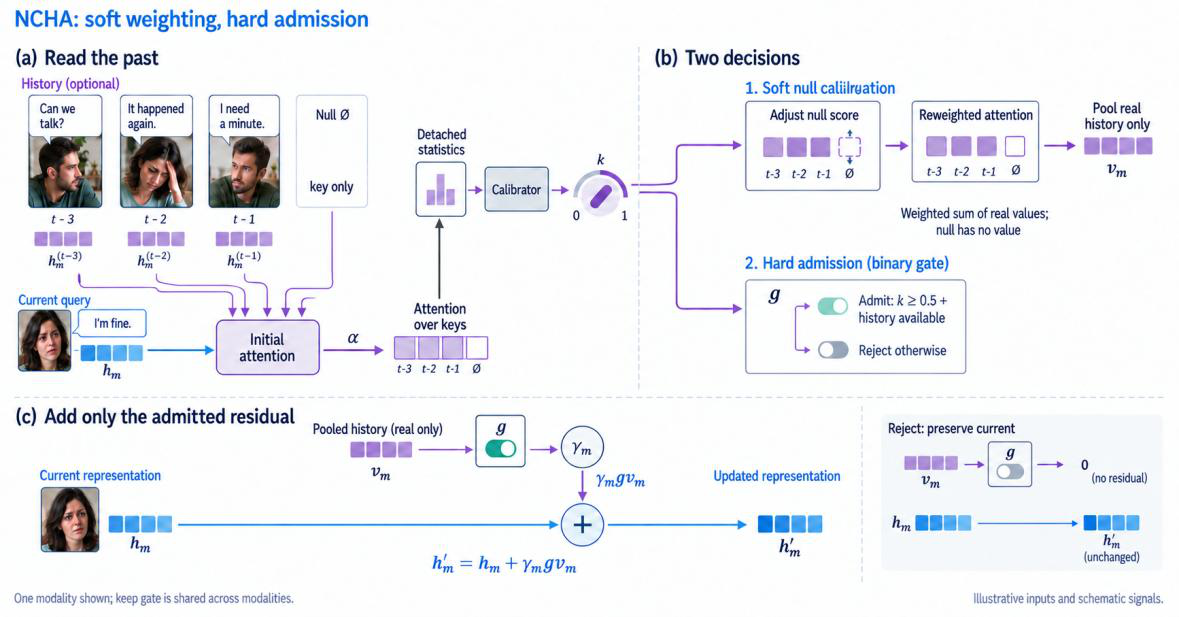
\includegraphics[width=0.94\linewidth]{figures/fig5_ncha.png}
  \caption{\textbf{NCHA null-candidate history abstention.}
  (a)~First pass: the current token estimates the relevance of the real historical slots.
  (b)~Second pass: a learned null candidate competes with the valid history; only real slots contribute value vectors.
  (c)~A utility-calibrated keep gate decides whether the historical update is applied at all, and rejected history is blocked from every downstream path.}
  \label{fig:ncha}
\end{figure}

Ordinary attention has no abstention option: even when all history is harmful, it still distributes probability over the available slots.
NCHA separates the \emph{selection} of historical content from the \emph{decision} to admit its update (Fig.~\ref{fig:ncha}).
A first attention pass estimates which real historical slots are relevant for each modality; a second pass adds one learned null candidate per modality and lets it compete with valid history.
Before feedback, a detached 24-dimensional feature vector summarizes the evidence available to the admission decision: current-utterance entropy, top-two margin, modality presence, history coverage, current-versus-history prediction divergence, history entropy, and speaker-related availability.
The keep gate, its bias and the admission indicator are
\begin{equation}
  k_t = \sigma(u_t / T_h), \qquad
  b_t = \beta\,[\log(1-k_t) - \log k_t],
  \label{eq:keepgate}
\end{equation}
\begin{equation}
  g_t = \ind[k_t \geq \theta]\;\ind[\Hist_t \text{ has valid slots}],
  \label{eq:admission}
\end{equation}
with $T_h{=}1$, $\beta{=}1$ and a hard threshold $\theta{=}0.5$; logarithm arguments are clamped at $10^{-5}$.
A high keep probability lowers the relative null score and lets real history compete normally; a low keep probability raises the null score and makes abstention likely.
Real history and the null candidate compete in the second normalization, but only real history contributes a value vector:
\begin{equation}
  s_{t\emptyset}^m = \frac{\langle W_q^m z_t^m,\, n_m\rangle}{\sqrt{d}} + b_t, \qquad
  \alpha_t^m = \softmax\big([s_{tj}^m]_{j\in\Hist_t},\, s_{t\emptyset}^m\big),
  \label{eq:nullattn}
\end{equation}
where $n_m$ is the learned null embedding and invalid historical scores are masked before normalization.
The null mass reduces the attention given to real history but never creates a synthetic feature vector, so rejected history cannot re-enter through another path; the same admission value also gates the optional memory path.
During training the hard decision is made differentiable with a straight-through estimator, while inference uses the binary gate directly:
\begin{equation}
  g_t^{\mathrm{ST}} = g_t + k_t - \sg(k_t).
  \label{eq:straightthrough}
\end{equation}
If a sample is rejected, the historical residual in Eq.~\eqref{eq:fccr} is set to zero for the whole utterance while the current encodings remain available.
No history label is required at test time: the decision uses only detached uncertainty, margin, availability, divergence and speaker-state features.

\subsection{Complementary evidence modeling with cRBEF}
\label{sec:crbef}

\begin{figure}[t]
  \centering
  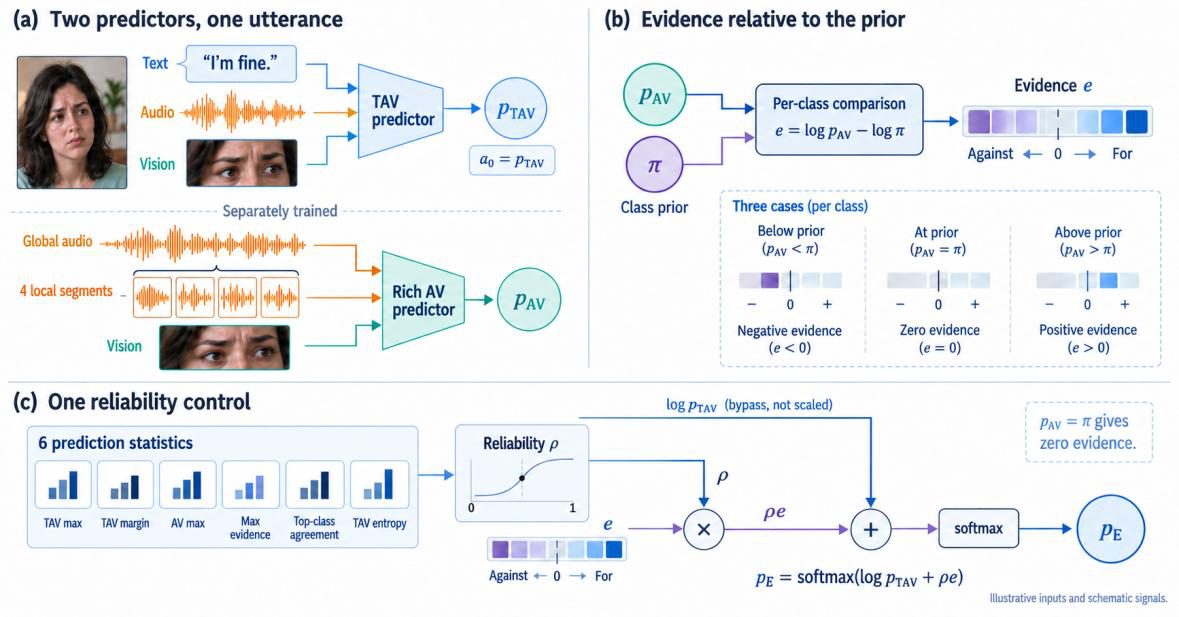
\includegraphics[width=0.94\linewidth]{figures/fig6_crbef.png}
  \caption{\textbf{cRBEF: prior-relative audio-visual evidence and reliability gating.}
  The TAV predictor (top) supplies the all-modality reference distribution; the text-free AV predictor (bottom) integrates global and local acoustic summaries with visual features.
  Class-wise evidence is the log ratio of the AV posterior to the stored class prior, a six-statistic gate scales it, and the gated evidence corrects the TAV log-probabilities before normalization.}
  \label{fig:crbef}
\end{figure}

A single MHnoU predictor can still be confidently wrong when lexical context dominates a nonverbal cue.
cRBEF provides a second, differently constructed opinion (Fig.~\ref{fig:crbef}).
It is loaded as a frozen external module that shares neither encoders nor router parameters with MHnoU, and contains a text--audio--visual (TAV) predictor, a separate text-free audio--visual (AV) predictor, and a six-input reliability gate.

The TAV predictor consumes the original cRBEF feature contract---a 4096-dimensional text vector, a 1024-dimensional audio vector and a 342-dimensional visual vector.\todo{cite the 342-d visual feature extractor (see M3ED feature docs).}
Audio and vision are independently projected to 256 dimensions, layer-normalized~\cite{ba2016layernorm}, masked by binary presence flags, and concatenated with text into a 4608-dimensional input; a linear layer reduces it to 128 dimensions, followed by GELU~\cite{hendrycks2016gelu}, dropout $0.2$, layer normalization, a seven-class head, and a learned tanh logit-temperature.
The AV predictor uses one global and four local 1024-dimensional acoustic summaries together with vision; global audio, flattened local audio and vision are each projected to 256 dimensions, layer-normalized, concatenated, and classified by a 128-dimensional head with the same structure.

A naive probability average cannot express class-specific support.
Let $p^{TAV}$ and $p^{AV}$ denote the two distributions and $\pi$ the stored training class prior.
For each class $c$, cRBEF forms prior-relative evidence $e_c = \log p^{AV}_c - \log \pi_c$: positive evidence means the AV branch supports class $c$ beyond its prior frequency, negative evidence the opposite.
The gate input $s$ has six components---the maximum TAV probability, its top-two margin, the maximum AV probability, the strongest prior-relative AV evidence, a binary top-class-agreement indicator, and the unnormalized TAV entropy---and a learned linear map with sigmoid produces the utterance-specific gate $\rho\in(0,1)$:
\begin{equation}
  e_c = \log p^{AV}_c - \log \pi_c, \qquad
  \rho = \sigma(v^{\top}s + b),
  \label{eq:evidence}
\end{equation}
\begin{equation}
  p^{E}_c = \frac{\exp(\log p^{TAV}_c + \rho e_c)}{\sum_{r=1}^{K}\exp(\log p^{TAV}_r + \rho e_r)}.
  \label{eq:expert}
\end{equation}
When $\rho\!\to\!0$ cRBEF reduces to the TAV reference; larger $\rho$ applies a stronger prior-relative correction, and because $e$ can be positive or negative, cRBEF can either strengthen or suppress a class.

\subsection{Bounded local class-wise fusion}
\label{sec:fusion}

\begin{figure}[t]
  \centering
  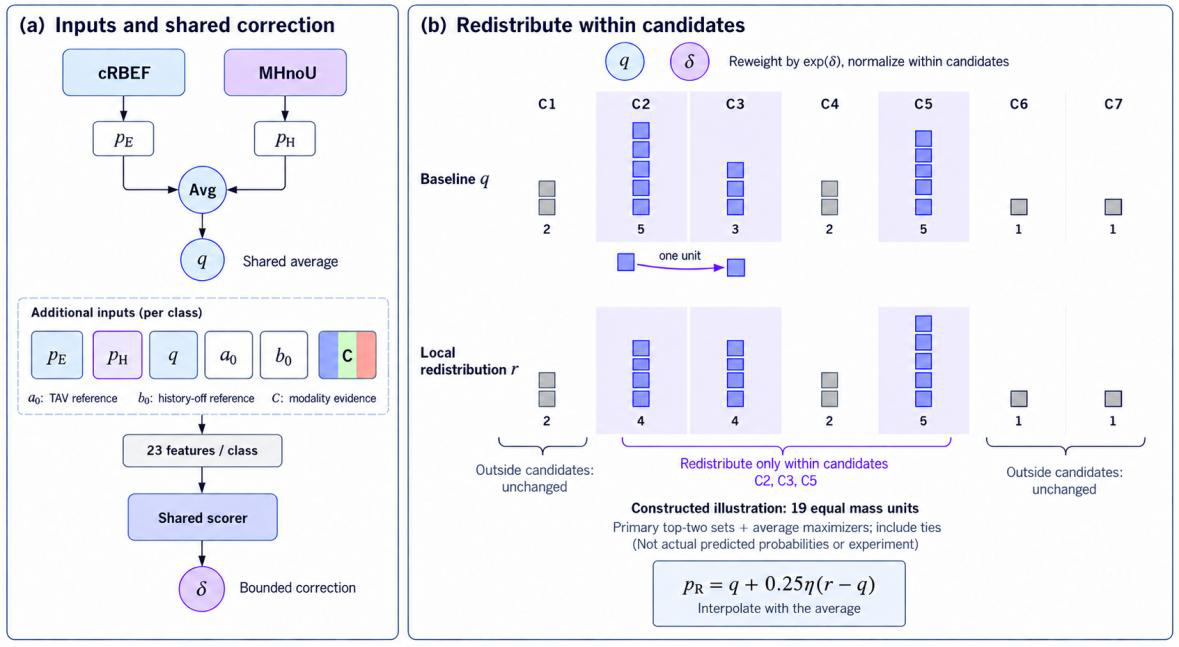
\includegraphics[width=0.94\linewidth]{figures/fig7_fusion.png}
  \caption{\textbf{Bounded local class-wise fusion and equal-weight fallback.}
  The two complete predictions and the two reference distributions form $P$; per-class features together with centered modality evidence feed a zero-initialized corrector whose bounded residual redistributes mass only inside a candidate set; the output interpolates with the equal-weight baseline, which is recovered exactly at $\eta=0$.}
  \label{fig:fusion}
\end{figure}

After obtaining two complete peer predictions, simple averaging cannot use the internal reference changes or the relative modality evidence to resolve a disagreement.
The outer fusion therefore uses two complete predictions and two reference distributions (Fig.~\ref{fig:fusion}):
\begin{equation}
  P = [a,\, b,\, a_0,\, b_0] = [p^{E},\, p^{H},\, p^{TAV},\, p^{H0}], \qquad q = (a+b)/2,
  \label{eq:baseline}
\end{equation}
where $a,b$ define the peer baseline and $a_0,b_0$ anchor changes from each internal reference; $p^{H0}$ is generated from the same MHnoU checkpoint with history masks zeroed.
The no-history auxiliary logits provide additional relative evidence: removing the class-wise mean logit within each modality and subtracting the cross-modality mean produces one centered evidence vector per modality in $C$, which records which modality relatively supports a class under the MHnoU checkpoint.
$C$ is not a second prediction and is never fed back into cRBEF.

For each class, the local corrector receives 23 features: the two primary probabilities, their logarithms, the baseline probability and its logarithm; the entropy and top-two margin of each primary; two top-class indicators; the two reference probabilities with their logarithms, their changes toward the complete predictions, and L1-normalized versions thereof; and the three centered evidence values of $C$.
Feature statistics are fitted only on the fusion set, clamped at $10^{-5}$, and standardized:
\begin{equation}
  \delta_c = 1.5\tanh\!\big(f_\psi(\clip((x_c - \bar{x})/s_x,\, -10,\, 10))\big),
  \label{eq:corrector}
\end{equation}
producing a bounded class-wise residual score.
The candidate set restricts correction to classes that already have local support---every class whose probability reaches at least the second-largest probability of either primary, plus the baseline argmax---and only mass inside this set is reallocated:
\begin{equation}
  B = \sum_{j\in\Kset} q_j, \qquad
  r_c = \frac{B\, q_c \exp(\delta_c)}{\sum_{j\in\Kset} q_j \exp(\delta_j)},\; c\in\Kset; \qquad
  r_c = q_c,\; c\notin\Kset.
  \label{eq:candidate}
\end{equation}
The final prediction interpolates between the corrected distribution and the equal-weight baseline:
\begin{equation}
  p^{R} = q + 0.25\,\eta\,(r - q), \qquad \eta \in [0,1].
  \label{eq:interp}
\end{equation}
$\eta=0$ recovers the baseline exactly; the last correction layer is zero-initialized, so an unfitted module is exactly the equal-probability baseline---a safe fallback when fitting does not improve the calibration split.

\subsection{Training and inference of ReCoMER}
\label{sec:training}

ReCoMER is trained in stages.
First, MHnoU is optimized with joint classification supervision and standardized Shapley regression:
\begin{equation}
  \mathcal{L}_{MH} = \mathrm{CE}_{\omega,\,0.05}(p^H, y) + 0.3\,\mathrm{MSE}(\mu, \hat{\phi}),
  \label{eq:lossmh}
\end{equation}
where cross-entropy uses label smoothing $0.05$ and class weights $\min\!\big(2, \sqrt{N/(K n_c)}\big)$ with class counts $n_c \geq 1$.
NCHA receives task gradients through historical feedback and its straight-through gate; no separate unimodal classification losses are used.
Second, with both prediction models frozen, only the outer corrector is fitted on ReCoMER's fused distribution $p^R$:
\begin{multline}
  \mathcal{L}_{F} = \frac{1}{N}\sum_{i=1}^{N}\Big[-\log p^{R}_{i,y_i} \\
    + 2 I_i \max\!\big(\log q_{i,y_i} - \log p^{R}_{i,y_i},\, 0\big)\Big]
    + 0.01\,\mean_{i,c}(\delta_{ic}^{2}),
  \label{eq:lossfusion}
\end{multline}
with $I_i = \ind\big[\argmaxop_c q_{ic} = y_i\big]$.
The preservation term discourages reducing true-class confidence on baseline-correct samples; fitting and strength selection use sample- and source-disjoint FIT and CAL sets, and $\eta$ is selected from $\{0, 0.25, 0.5, 1\}$ by weighted F1 on CAL.

The current bundle implements seven-class M3ED recognition.
MHnoU uses 192-dimensional embeddings, a two-layer six-head Transformer (feed-forward width 576), dropout $0.15$, and up to three historical slots; its text, audio and vision input dimensions are 2560, 2048 and 342.
Both stages use AdamW~\cite{loshchilov2019adamw} (learning rates $2{\times}10^{-4}$ and $10^{-3}$, weight decay $0.01$; 40 epochs for the corrector).
At inference, MHnoU produces $p^H$ and, with history masks disabled, $p^{H0}$ and auxiliary modality evidence; cRBEF produces $p^E$ and its TAV reference.
The framework aligns these outputs, constructs $P$ and $C$, applies Eqs.~\eqref{eq:baseline}--\eqref{eq:interp}, and returns the argmax of $p^R$.
No class or history labels enter this inference path.

%%%%%%%%% 4. EXPERIMENTS
\section{Experiments}
\label{sec:experiments}

\subsection{Experimental setup}
\label{sec:setup}

We evaluate ReCoMER with five complementary evidence sources---a frozen formal test of the complete system, module-isolation studies for the three components, corrected abstention experiments, an exact-feature replication of the cRBEF expert, and cross-dataset instantiations on IEMOCAP and MELD---which use different splits, seeds, and fusion scopes.

\paragraph{Datasets, metrics and protocols.}
We use MELD~\cite{poria2019meld}, M3ED~\cite{zhao2022m3ed} and IEMOCAP~\cite{busso2008iemocap} for classification (weighted F1, WF1, higher is better) and CMU-MOSEI~\cite{zadeh2018cmumosei} for regression (MAE, lower is better).
The module-isolation studies use ten seeds (7, 13, 17, 23, 29, 37, 43, 53, 71, 101); the abstention study uses three seeds under the corrected protocol; the frozen formal ReCoMER test consists of three paired runs with the cRBEF checkpoint fixed at seed 17; the exact-feature M3ED queue uses ten seeds for MHnoU controls and five for the standalone cRBEF replication.
Capacity and optimization settings follow Sec.~\ref{sec:method}; the formal runs use batch size 256 and early stopping on the selection split.
The exact M3ED HuBERT feature pack~\cite{hsu2021hubert} contains 17{,}427/2{,}821/4{,}201 train/validation/test samples (feature dimensions 768/2048/342; text from a BERT pack~\cite{devlin2019bert}).
Test data were not used for model or module selection; the formal test was opened only after all controls had been frozen, and confidence intervals in the module-isolation studies are paired seed-level intervals on fixed validation protocols, whereas those in the formal test are dialogue-bootstrap intervals over test conversations; the two are not interchangeable.

\subsection{Main comparison on the frozen M3ED test}
\label{sec:main}





\begin{figure*}[t]
  \centering
  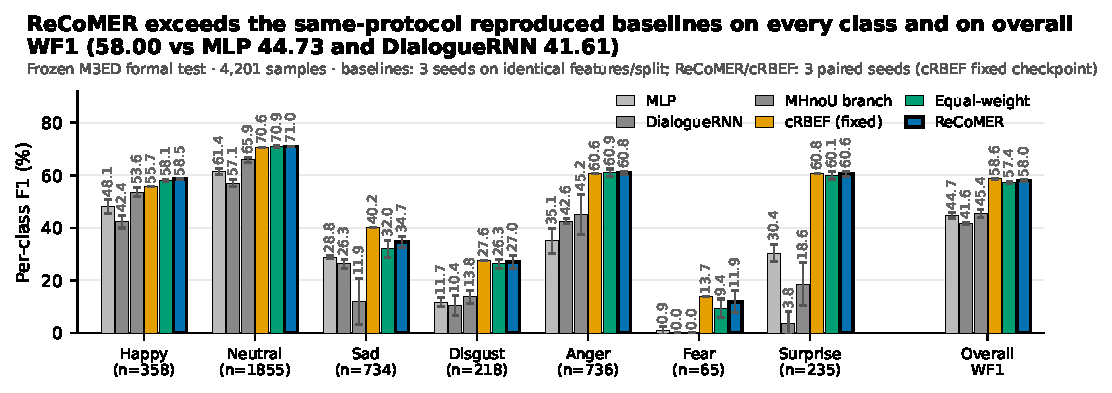
\includegraphics[width=\textwidth]{figures/figE_perclass_with_baselines.pdf}
  \caption{\textbf{ReCoMER exceeds the same-protocol reproduced baselines on every class and overall.}
  Per-class and overall WF1 (rightmost group) on the frozen M3ED formal test, mean $\pm$ SD over three paired seeds; MLP and DialogueRNN reproduced on identical features and split; cRBEF checkpoint fixed; AV/TAV are its internal branches (48.71/57.03).}
  \label{fig:combined}
\end{figure*}



Fig.~\ref{fig:combined} compares the complete system with its fusion controls and with two same-protocol reproduced references, overall (rightmost group) and per class.
ReCoMER improves over matched equal weight by $0.607$ points (95\% CI $[0.250, 1.005]$), exceeds the reproduced MLP and DialogueRNN by $13.3$ and $16.4$ points on identical features/split, and attains the best accuracy and calibration among all fusion rules (appendix Fig.~\ref{fig:multimetric}); these entry-level references are not a SOTA claim; the $51.66$\% DialogueRNN of the M3ED paper~\cite{zhao2022m3ed}, under different features, shows the protocol sensitivity of this benchmark.
The fixed cRBEF expert---a frozen \emph{input} of the system, not a competitor---remains $0.60$ points above the complete system, and a sample-level decomposition (appendix Fig.~\ref{fig:gapdecomp}) shows that the bounded correction recovers $0.5$--$1.0$ points over equal weight with zero collateral errors but cannot rescue the $359$ disputed samples where the branch is confidently wrong (concentrated in Sad and Anger), and that one of three seeds calibrated to $\eta{=}0$.
The gap is attributable to branch quality on minority classes rather than to the fusion rule.
Per class (Fig.~\ref{fig:combined}, bottom), ReCoMER exceeds both reproduced baselines on all seven classes; against the expert it trades Sad for Happy and Fear.



\subsection{Component isolation studies}
\label{sec:isolation}



\paragraph{Historical feedback.}
Under uniform modality weights (appendix Table~\ref{tab:history}), history gives the clearest gain on MOSEI, a positive M3ED effect that misses the pre-specified 8/10 criterion, and a MELD interval crossing zero; ordering controls overlap zero, supporting conditional historical-feedback fusion.



\paragraph{Contribution routing.}
With the encoder, history module, solo heads and joint head frozen, only the EvidenceRouter utility head was optimized on a fixed uniform backbone with exact per-sample Shapley supervision (appendix Table~\ref{tab:router} and Fig.~\ref{fig:routerforest}).
The router improves MOSEI MAE significantly against all three controls (10/10 seeds, Holm $p{=}0.006$); on MELD it beats the uniform prior (8/10) but only marginally after correction, and on M3ED it is neutral against the uniform prior; routing helps when modalities provide complementary evidence.


\paragraph{History abstention.}
The third study lets the model choose between real historical candidates and an explicit empty candidate (variants in appendix Table~\ref{tab:abstain}): the utility-calibrated variant improves IEMOCAP WF1 by $0.61$ and reduces MOSEI MAE by $0.0013$, is unchanged on MELD, and decreases M3ED WF1 by $0.28$; the other variants show no stable advantage---a dataset-dependent abstention effect.

\subsection{Integrated ablations and information-flow checks}
\label{sec:ablation}




Appendix Table~\ref{tab:ablation} reports paired ablations: the full model beats equal weighting, removing history abstention is harmful, and the remaining intervals overlap zero (mechanism indications).
The cRBEF/MHnoU splice passes all identity and information-flow checks, confirming cRBEF as an external expert rather than an accidental input to the MHnoU router.

\subsection{Ten-seed controlled matrix across four datasets}
\label{sec:exact}



A controlled ten-seed matrix over all four datasets on the model6 feature stack with valid-based selection separates model behavior from feature-protocol effects (appendix Table~\ref{tab:matrix4}).
The evidence router with solo-weighted deployment is the only arm that improves consistently---significant gains over the matched controls on the three classification datasets (all 10/10 seeds, Holm $p{\le}0.002$) and the best mean MAE on MOSEI---whereas the closed-loop deployment is not significant on any dataset.
These valid-split diagnostics must not be merged with the $58.00$\% formal test result; an M3ED-only exact-pack queue reaches $0.5399$ versus B0 at $0.5353$ (appendix Table~\ref{tab:exact}).

\subsection{Cross-dataset instantiation}
\label{sec:transfer}





To test instantiation beyond the development benchmark, we rebuilt the expert per dataset on the IEMOCAP and MELD packs and fused it with the MHnoU branch through the same reliability-gated fusion (fixed-$\alpha$ gate from valid; three seeds).
On IEMOCAP (4-class; Qwen3 text pack) the fused system reaches $73.73$, above the strongest expert arm ($72.95$) and equal weight ($72.51$), the gain positive in all three seeds ($+1.74/+0.47/+0.14$, mean $+0.8$ pp);
on MELD (7-class; $T{=}1024$ text pack) it improves over equal weight ($65.32$) and the branch ($65.06$), matches the gated expert ($65.75$), and stays $0.4$ points below the text-only expert ($66.16$).
Across the three datasets (appendix Fig.~\ref{fig:transfer}), fusion adds value when branch and expert are comparably strong and degrades gracefully otherwise; the instances use a fixed-$\alpha$ gate rather than the learned local corrector, and the 4-class IEMOCAP instance is not comparable to 6-class ERC results.

\subsection{Failure boundaries and reproducibility}
\label{sec:limits}


Three scope conditions emerge: M3ED is strong at the utterance level, so history feedback and routing have small or negative marginal effects; in a subgroup analysis (appendix Fig.~\ref{fig:subgroup}) history feedback helps continuation utterances in all nine dataset$\times$seed pairs but is consistently harmful on M3ED label flips (3/3 seeds) and neutral elsewhere, so transition risk is dataset-dependent; and MOSEI benefits most from historical compensation, though the direction is metric-specific.
The run package records hashes, checkpoints, per-seed histories, Shapley diagnostics, weights, decisions, masks and split guards.
A same-protocol comparison with stronger systems remains pending (the reproduced references in Fig.~\ref{fig:combined} are entry-level, not SOTA).



%%%%%%%%% 5. CONCLUSION
\section{Conclusion}
\label{sec:conclusion}

ReCoMER answers the varying reliability of historical context and individual modalities with a conditional-fusion framework whose separation makes the information flow auditable and each component independently testable.
On the frozen formal M3ED test it reaches $58.00$\% WF1, $0.607$ points above matched equal-weight fusion and $13$--$16$ points above same-protocol reproduced references, and cross-dataset instantiations confirm that its conservative gate fusion adds value when branch and expert are matched and degrades gracefully otherwise.
The evidence supports conditional, evidence-dependent gains; future work will upgrade the MELD text contract, complete same-protocol comparisons with stronger systems, and close the branch--expert strength gap.

%%%%%%%%% REFERENCES
{
  \small
  \bibliographystyle{ieeenat_fullname}
  \bibliography{refs}
}

%%%%%%%%% APPENDIX (move to a separate supplementary file for submission)
\appendix
\section{Supplementary diagnostics}
\label{sec:appendix}


\begin{table}[h]
  \centering
  \caption{\textbf{Integrated ReCoMER ablations.}
  Full $-$ control in percentage points of test WF1.}
  \label{tab:ablation}
  \small
  \setlength{\tabcolsep}{4pt}
  \begin{tabular}{lcc}
    \toprule
    Control & Full $-$ control & Dialogue-bootstrap 95\% CI \\
    \midrule
    Equal-weight fusion & $+0.607$ & [$0.250$, $1.005$] \\
    No relative contribution $C$ & $+0.013$ & [$-0.043$, $0.069$] \\
    No Shapley supervision & $-0.050$ & [$-0.281$, $0.158$] \\
    Unbounded softmax weights & $-0.036$ & [$-0.272$, $0.172$] \\
    No history abstention & $-0.487$ & [$-0.911$, $-0.091$] \\
    No contribution-token feedback & $-0.015$ & [$-0.290$, $0.248$] \\
    No history-residual feedback & $-0.056$ & [$-0.160$, $0.047$] \\
    \bottomrule
  \end{tabular}
\end{table}

\begin{table}[h]
  \centering
  \caption{\textbf{Historical feedback under ten-seed validation protocols.}
  Positive values indicate improved WF1 or reduced MAE, following the metric direction.}
  \label{tab:history}
  \small
  \begin{tabular}{llccc}
    \toprule
    Dataset & Metric & Mean effect & 95\% CI & Seeds \\
    \midrule
    M3ED & WF1 $\uparrow$ & $+0.0048$ & [$+0.0011$, $+0.0084$] & 7/10 \\
    MELD & WF1 $\uparrow$ & $-0.0015$ & [$-0.0082$, $+0.0052$] & 5/10 \\
    MOSEI & MAE $\downarrow$ & $+0.0034$ & [$+0.0000$, $+0.0067$] & 8/10 \\
    \bottomrule
  \end{tabular}
\end{table}

\begin{table}[h]
  \centering
  \caption{\textbf{Corrected history-abstention variants.}
  B1: original empty-candidate design; E5: adds utility calibration before softmax normalization; E6: additionally uses semantic history features; E7: replaces softmax with sparsemax~\cite{martins2016sparsemax}.
  Mean $\pm$ population standard deviation over three seeds. Metrics: MELD dev WF1 $\uparrow$; M3ED and IEMOCAP val WF1 $\uparrow$; MOSEI val MAE $\downarrow$.}
  \label{tab:abstain}
  \scriptsize
  \setlength{\tabcolsep}{4pt}
  \begin{tabular}{lcccc}
    \toprule
    Variant & MELD & M3ED & IEMOCAP & MOSEI \\
    \midrule
    B1 & $0.5967{\pm}.007$ & $0.5610{\pm}.001$ & $0.7248{\pm}.002$ & $0.5640{\pm}.003$ \\
    E5 & $0.5970{\pm}.009$ & $0.5583{\pm}.001$ & $0.7309{\pm}.007$ & $0.5627{\pm}.003$ \\
    E6 & $0.5968{\pm}.009$ & $0.5583{\pm}.001$ & $0.7309{\pm}.007$ & $0.5627{\pm}.003$ \\
    E7 & $0.5957{\pm}.009$ & $0.5587{\pm}.002$ & $0.7304{\pm}.006$ & $0.5633{\pm}.003$ \\
    \bottomrule
  \end{tabular}
\end{table}

\begin{table}[h]
  \centering
  \caption{\textbf{Four-dataset controlled matrix (ten seeds, valid selection, model6 feature stack).}
  Mean $\pm$ SD of valid WF1 (\%, $\uparrow$) for M3ED/MELD/IEMOCAP and valid MAE ($\downarrow$) for MOSEI.
  B0 = uniform weights without history; solo = evidence router with solo-weighted deployment.
  Paired seed-level results for solo: $+1.50$ pp vs B0 on M3ED (10/10, $p{=}0.002$); $+0.75$ pp vs uniform-history on MELD (10/10, $p{=}0.002$); $+1.20$ pp vs B0 on IEMOCAP (10/10, $p{=}0.002$); best mean MAE on MOSEI (8/10).}
  \label{tab:matrix4}
  \scriptsize
  \setlength{\tabcolsep}{3.5pt}
  \resizebox{\columnwidth}{!}{%
  \begin{tabular}{lcccc}
    \toprule
    Arm & M3ED & MELD & IEMOCAP & MOSEI \\
    \midrule
    B0 (uniform, no history) & $58.80{\pm}0.44$ & $63.47{\pm}0.40$ & $68.54{\pm}0.97$ & $0.5108{\pm}0.0039$ \\
    Uniform + history & $59.01{\pm}0.50$ & $63.34{\pm}0.27$ & $68.95{\pm}0.64$ & $0.5091{\pm}0.0043$ \\
    Evidence (closed loop) & $58.96{\pm}0.34$ & $63.38{\pm}0.23$ & $68.91{\pm}1.07$ & $0.5090{\pm}0.0047$ \\
    \textbf{Evidence (solo-weighted)} & $\mathbf{60.30{\pm}0.45}$ & $\mathbf{64.09{\pm}0.34}$ & $\mathbf{69.73{\pm}0.58}$ & $\mathbf{0.5068{\pm}0.0056}$ \\
    Evidence + memory path & $59.20{\pm}0.40$ & $63.45{\pm}0.21$ & $69.20{\pm}0.88$ & $0.5112{\pm}0.0056$ \\
    \bottomrule
  \end{tabular}}
\end{table}

\begin{table}[h]
  \centering
  \caption{\textbf{Exact-feature M3ED ten-seed test controls.}}
  \label{tab:exact}
  \small
  \begin{tabular}{lc}
    \toprule
    Arm & Test WF1 \\
    \midrule
    Uniform, no history (B0) & $0.5353 \pm 0.0058$ \\
    Uniform + history & $0.5346 \pm 0.0049$ \\
    Evidence (closed loop) & $0.5373 \pm 0.0041$ \\
    Evidence + memory path & $0.5399 \pm 0.0064$ \\
    Uniform + abstention & $0.5339 \pm 0.0049$ \\
    \bottomrule
  \end{tabular}
\end{table}


\begin{table}[h]
  \centering
  \caption{\textbf{EvidenceRouter under the fixed-backbone ten-seed protocol.}
  Change = router minus control (percentage points, or MAE$\times$100 for MOSEI); wins = seeds with improvement; Holm $p$ over the full comparison family.}
  \label{tab:router}
  \scriptsize
  \setlength{\tabcolsep}{3.5pt}
  \begin{tabular}{llccc}
    \toprule
    Dataset & Control & Change [95\% CI] & Wins & Holm $p$ \\
    \midrule
    \multirow{3}{*}{MOSEI $\downarrow$}
      & uniform & $+0.67$ [$+0.49$, $+0.85$] & 10/10 & $0.006^{**}$ \\
      & constant task & $+0.51$ [$+0.27$, $+0.74$] & 10/10 & $0.006^{**}$ \\
      & MLP task & $+0.45$ [$+0.21$, $+0.70$] & 10/10 & $0.006^{**}$ \\
    \multirow{3}{*}{MELD $\uparrow$}
      & uniform & $+0.34$ [$+0.09$, $+0.59$] & 8/10 & $0.059$\,\textdagger \\
      & constant task & $+0.51$ [$+0.00$, $+1.01$] & 7/10 & $0.152$ \\
      & MLP task & $-0.04$ [$-0.36$, $+0.29$] & 4/10 & $0.824$ \\
    \multirow{3}{*}{M3ED $\uparrow$}
      & uniform & $-0.33$ [$-0.54$, $-0.12$] & 2/10 & $0.059$\,\textdagger \\
      & constant task & $+0.42$ [$+0.21$, $+0.63$] & 10/10 & $0.012^{*}$ \\
      & MLP task & $+0.09$ [$-0.09$, $+0.26$] & 6/10 & $0.613$ \\
    \bottomrule
  \end{tabular}
  \vspace{2pt}
  \raggedright\footnotesize $^{**}p<0.01$, $^{*}p<0.05$, \textdagger$~p<0.10$; verdicts visualized in appendix Fig.~\ref{fig:routerforest}.
\end{table}

\begin{figure}[h]
  \centering
  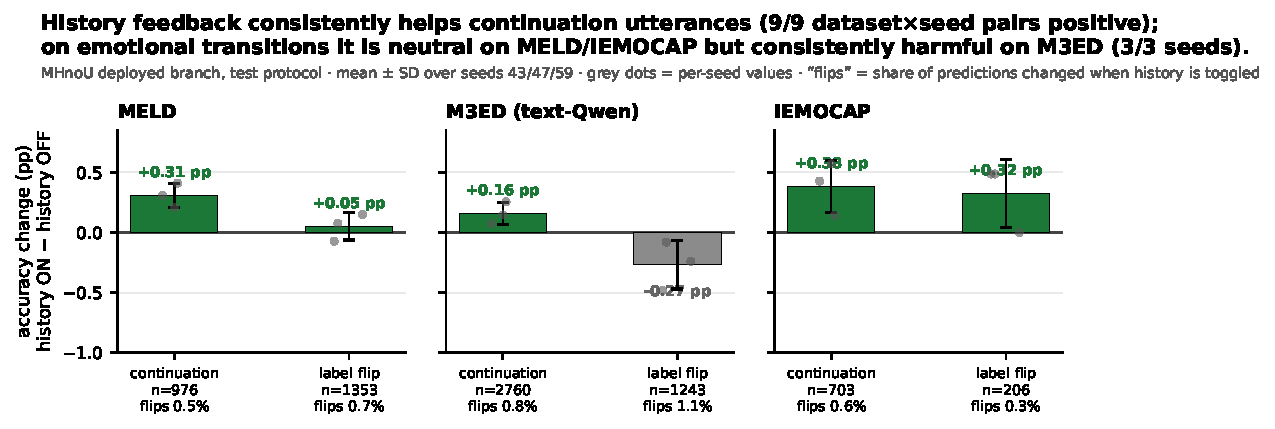
\includegraphics[width=\linewidth]{figures/figF_subgroup_transition.pdf}
  \caption{\textbf{History feedback consistently helps continuation utterances (9/9 dataset$\times$seed pairs positive); on emotional transitions it is neutral on MELD/IEMOCAP but consistently harmful on M3ED (3/3 seeds).}
  MHnoU deployed branch, test protocol; accuracy change (pp) between history on and off, mean $\pm$ SD over seeds 43/47/59; grey dots are per-seed values; ``flips'' is the share of predictions changed when history is toggled.}
  \label{fig:subgroup}
\end{figure}

\begin{figure}[h]
  \centering
  \begin{minipage}{0.46\linewidth}\centering
    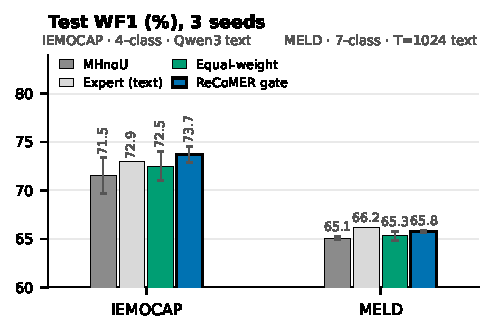
\includegraphics[width=\linewidth]{figures/figH_left_bars.pdf}
  \end{minipage}\hfill
  \begin{minipage}{0.46\linewidth}\centering
    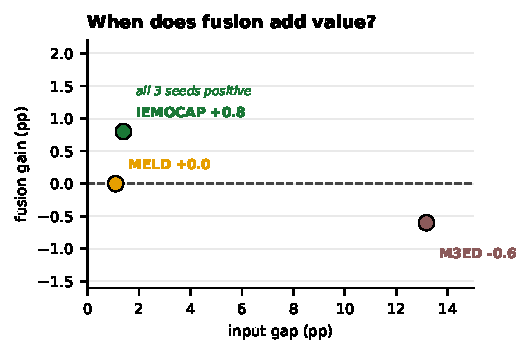
\includegraphics[width=\linewidth]{figures/figH_right_scatter.pdf}
  \end{minipage}
  \caption{\textbf{Cross-dataset instantiation: the conservative gate fusion adds value when branch and expert are matched (IEMOCAP, $+0.8$ pp over three seeds) and degrades gracefully when they are not (MELD, M3ED).}
  (a) Test WF1 (mean $\pm$ SD over three seeds) with a fixed-$\alpha$ gate ($\alpha$ from valid; the expert arm is a single checkpoint without seed variance).
  (b) Fusion gain over the strongest expert versus the input-strength gap (strongest expert minus branch); the M3ED point is the frozen formal test.}
  \label{fig:transfer}
\end{figure}

\begin{figure}[h]
  \centering
  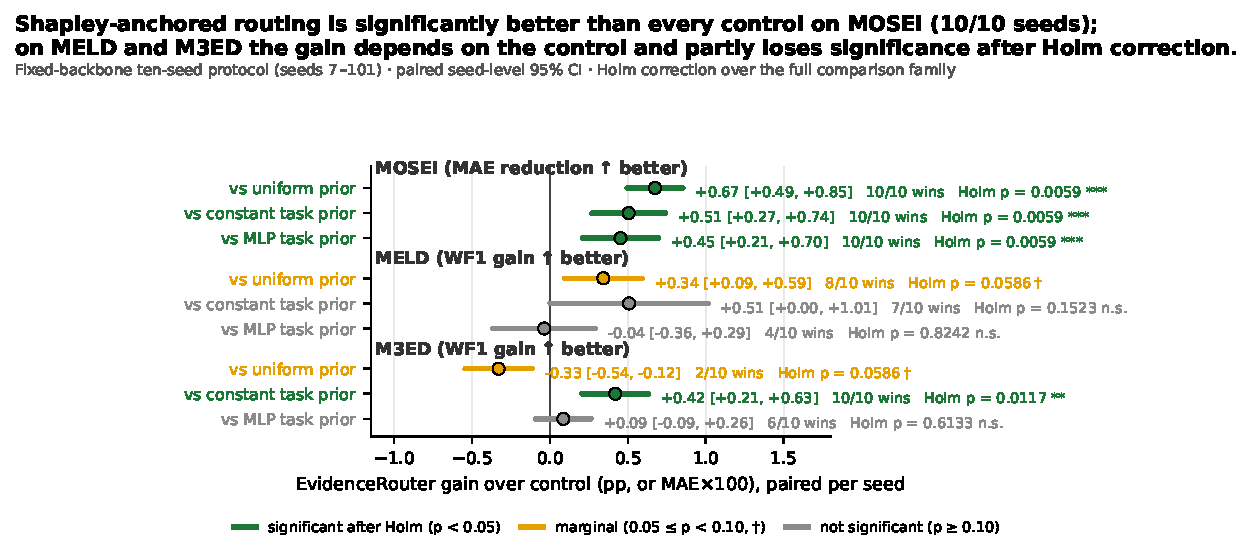
\includegraphics[width=\linewidth]{figures/figB_router_forest_holm.pdf}
  \caption{\textbf{Router gains as a Holm-corrected forest plot.}
  Fixed-backbone ten-seed protocol (seeds 7--101); paired seed-level 95\% CI; point color marks the Holm-corrected verdict (green $p<0.05$, amber $p<0.10$, grey not significant). Numerical values in Table~\ref{tab:router}.}
  \label{fig:routerforest}
\end{figure}


\begin{figure}[h]
  \centering
  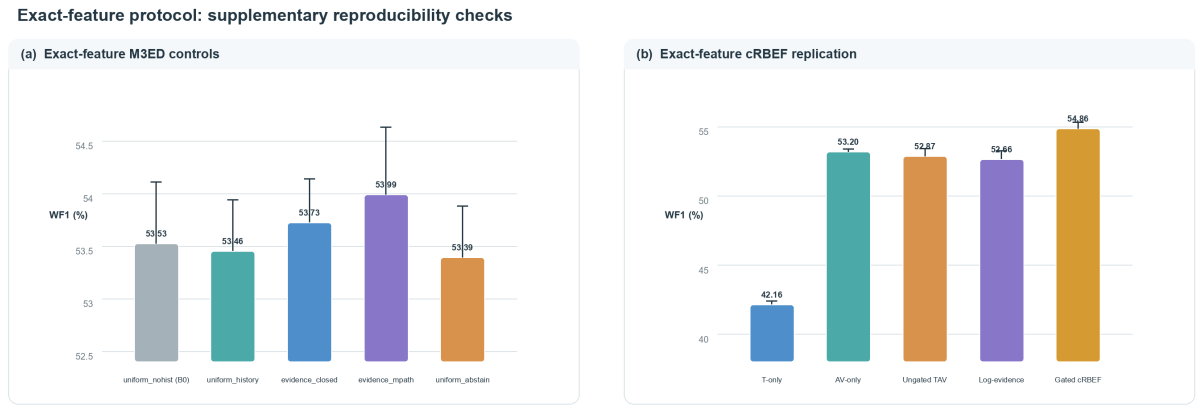
\includegraphics[width=\linewidth]{figures/fig9_exact_controls.png}
  \caption{\textbf{Exact-feature M3ED controls and cRBEF replication.}
  Left: ten-seed test WF1 of the five MHnoU control arms under the official M3ED split and feature pack.
  Right: five-seed replication of the cRBEF evidence heads on the exact T/A/V features, comparing T-only, AV-only, ungated and gated variants.}
  \label{fig:exact}
\end{figure}

\begin{figure}[h]
  \centering
  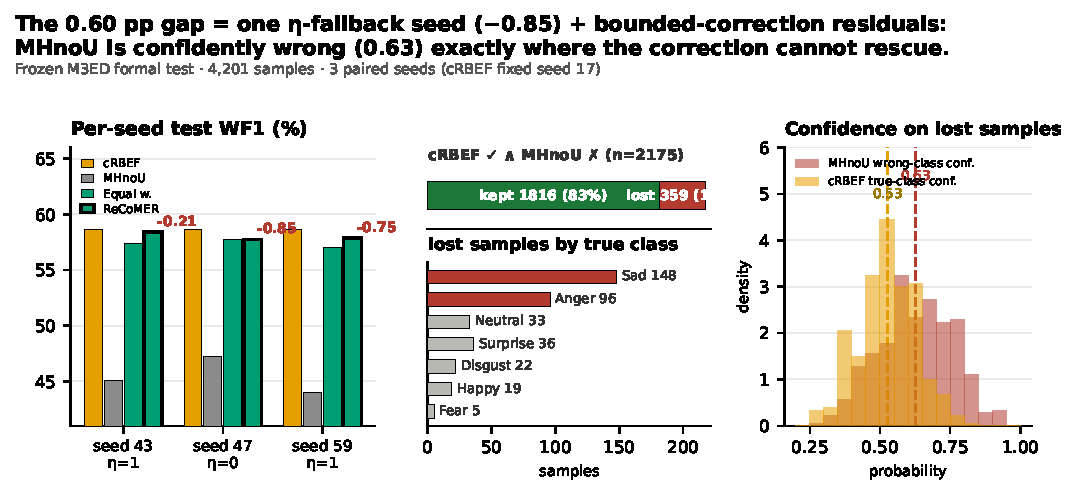
\includegraphics[width=\linewidth]{figures/figG_crbef_gap_decomposition.pdf}
  \caption{\textbf{Where the $0.60$ pp expert--system gap comes from.}
  Left: per-seed test WF1 of the four evaluated branches ($\eta$ annotated).
  Middle: disputed samples (expert correct, branch wrong): equal weight keeps 76\%, ReCoMER 84\%, with zero collateral errors; lost samples concentrate in Sad and Anger.
  Right: on lost samples the branch's wrong-class confidence (0.63) exceeds the expert's true-class confidence (0.53), beyond the bounded correction's reach.}
  \label{fig:gapdecomp}
\end{figure}

\begin{figure}[h]
  \centering
  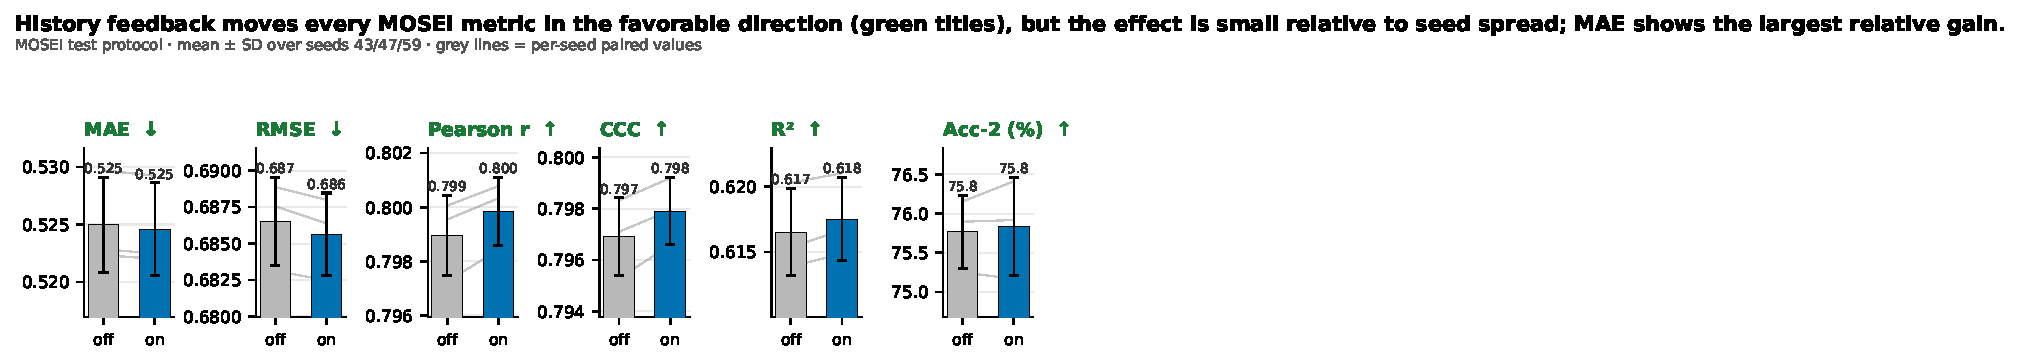
\includegraphics[width=\linewidth]{figures/figC_mosei_metric_profile.pdf}
  \caption{\textbf{History feedback moves every MOSEI metric in the favorable direction, but the effect is smaller than the seed spread.}
  MOSEI test protocol; mean $\pm$ SD over seeds 43/47/59; grey lines connect per-seed paired values; green titles mark the favorable direction.}
  \label{fig:moseiprofile}
\end{figure}

\begin{figure}[h]
  \centering
  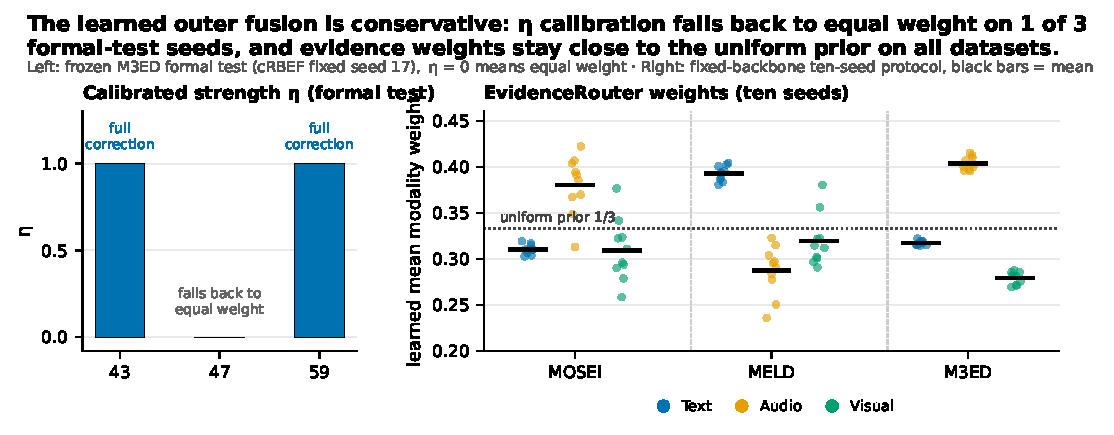
\includegraphics[width=\linewidth]{figures/figD_fusion_behavior.pdf}
  \caption{\textbf{The learned outer fusion is conservative.}
  Left: calibrated strength $\eta$ per formal-test seed ($\eta{=}0$ means the calibration set selected equal weight).
  Right: evidence-router modality weights across ten seeds stay close to the uniform prior; black bars are means.}
  \label{fig:fusionbehavior}
\end{figure}

\begin{figure}[h]
  \centering
  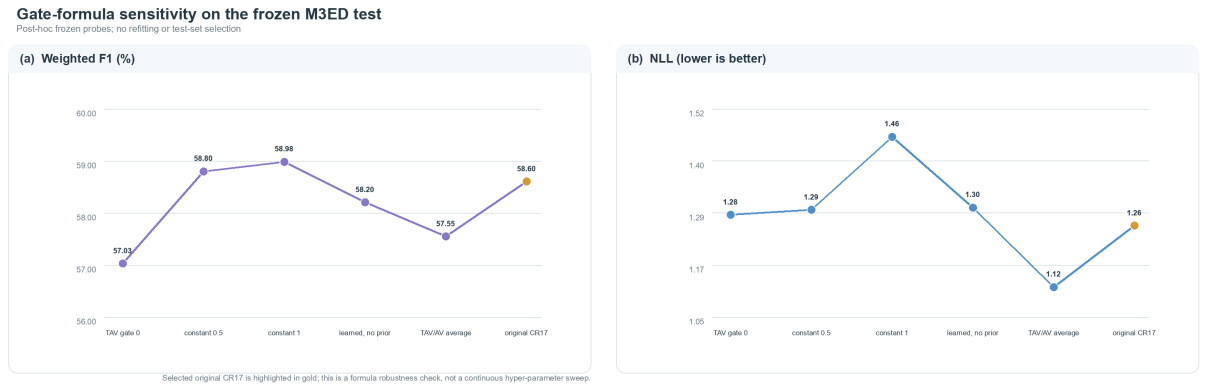
\includegraphics[width=\linewidth]{figures/fig10_sensitivity.png}
  \caption{\textbf{Frozen cRBEF gate-formula sensitivity.}
  A discrete formula-robustness check (not a continuous hyperparameter sweep): each bar shows the test WF1 obtained when one term of the gate formula is replaced by an alternative, with all other components frozen.}
  \label{fig:sensitivity}
\end{figure}

\begin{figure}[h]
  \centering
  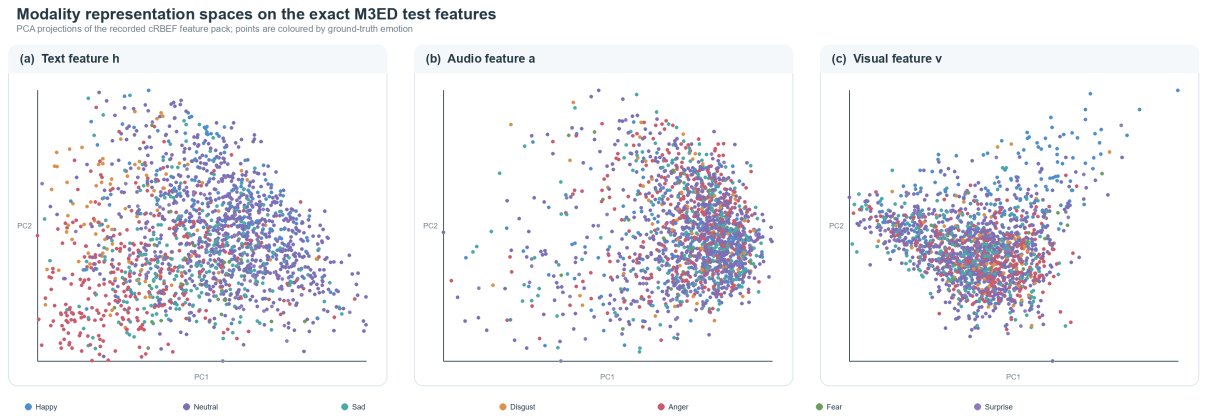
\includegraphics[width=\linewidth]{figures/fig11_pca.png}
  \caption{\textbf{PCA projections of exact M3ED test features.}
  Text, audio and vision features projected to two principal components and colored by ground-truth emotion, illustrating the very different class geometry available to each modality.}
  \label{fig:pca}
\end{figure}

\begin{figure}[h]
  \centering
  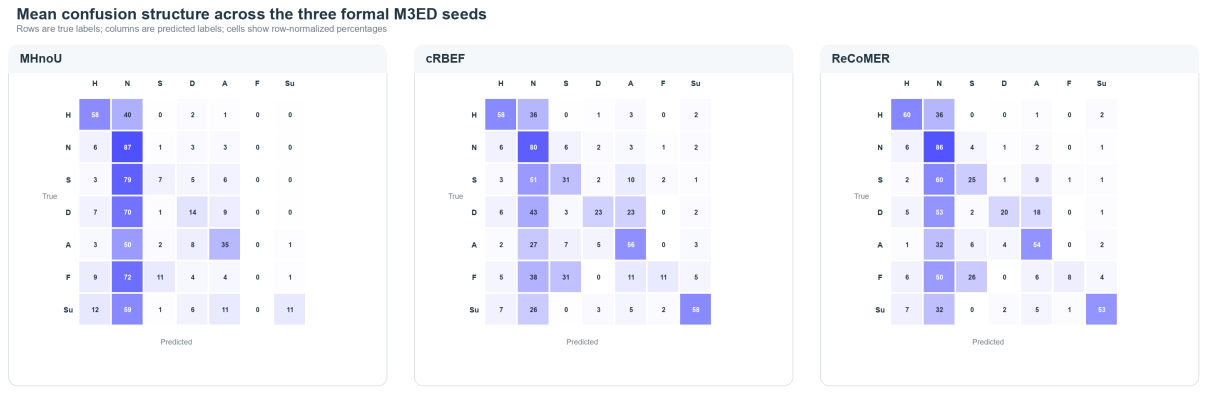
\includegraphics[width=\linewidth]{figures/fig12_confusion.png}
  \caption{\textbf{Mean row-normalized confusion structure.}
  Confusion matrices of MHnoU, cRBEF and ReCoMER averaged over the three formal M3ED test seeds, showing which emotion pairs each model confuses and how the fused system redistributes errors.}
  \label{fig:confusion}
\end{figure}

\end{document}
